\documentclass[11pt,a4paper]{article}

% ============ PAQUETES ============
\usepackage[utf8]{inputenc}
\usepackage[T1]{fontenc}
\usepackage{amsmath, amssymb}
\usepackage{graphicx}
\usepackage{geometry}
\usepackage{tikz}
\usetikzlibrary{positioning, arrows.meta}
\usepackage{booktabs}
\usepackage{array}
\usepackage{tabularx}
\usepackage{enumitem}
\usepackage{hyperref}
\usepackage{algorithm}
\usepackage{algpseudocode}
\usepackage{xcolor}
\usepackage{fancyhdr}
\usepackage{listings}
\usepackage{tocloft}

\renewcommand{\abstractname}{Resumen}
\renewcommand{\contentsname}{Índice}

\geometry{margin=2.5cm}
\hypersetup{colorlinks=true, linkcolor=blue, urlcolor=blue, citecolor=blue}

\pagestyle{fancy}
\fancyhf{}
\lhead{Algoritmos Avanzados -- Informe, Segunda Entrega}
\rhead{Grupo 1 -- Cobertura de Vértices}
\cfoot{\thepage}

\lstset{
	basicstyle=\ttfamily\small,
	breaklines=true,
	frame=single,
	columns=fullflexible,
	backgroundcolor=\color{gray!8}
}

% ============ DATOS DEL PROYECTO ============
\title{
	\vspace{-1cm}
	\textbf{Optimización de la Ubicación de Sistemas de Detección de Intrusos (IDS) \\
	mediante Cobertura de Vértices (Vertex Cover)} \\
	\large Informe Técnico de la Segunda Entrega: Implementación Funcional Completa, Escalabilidad en Redes Reales de Internet (Stanford SNAP), Interfaz Gráfica Interactiva y Análisis Experimental
}
\author{
	\textbf{Grupo 1} \\
	\small Universidad Nacional de San Antonio Abad del Cusco \\
	\small Facultad de Ingeniería Eléctrica, Electrónica, Informática y Mecánica \\
	\small Escuela Profesional de Ingeniería Informática y de Sistemas \\
	\small Asignatura: Algoritmos Avanzados \\
	\small Docente: Héctor Eduardo Ugarte Rojas \\
	\small Atributo del Graduado Evaluado: AG\_C06 -- Aprendizaje a lo largo de la vida \\
	\small Integrantes: \\
	\small Steffano Ricardo Caballero Zegarra \quad Adriel Alfredo Llactahuamani Ayala \\
	\small Albert Erik Morocco Amanca \quad Diego Alonso Quispe Castilla
}
\date{Semestre académico 2026-2 \\ Informe de la Segunda Entrega (Avances 4 y 5)}

\begin{document}

\maketitle
\thispagestyle{fancy}

\begin{abstract}
\noindent
El presente informe documenta el cumplimiento integral de los requerimientos para la \textbf{Segunda Entrega} del proyecto semestral de Algoritmos Avanzados, enfocado en la resolución, análisis y evaluación experimental del problema de Cobertura de Vértices (\textit{Vertex Cover}) aplicado a la ubicación costo-eficiente de Sistemas de Detección de Intrusos (IDS) en redes de comunicaciones. En esta fase se consolidó la transición desde el prototipo preliminar de la Primera Entrega hacia un sistema computacional completamente funcional, optimizado y escalable a topologías reales masivas. Específicamente, se rediseñó la heurística voraz implementando una cola de prioridad basada en montículos de máximos con actualización perezosa (\textit{Lazy Max-Heap}), reduciendo su complejidad de $O(V \cdot E)$ a $O((V+E)\log V)$ con desempate canónico determinístico; se mantuvo y optimizó la 2-aproximación por Emparejamiento Maximal (\textit{Maximal Matching}) en $O(V+E)$; se formuló y resolvió el problema exacto mediante Programación Lineal Entera (ILP); y se diseñó de manera autónoma un motor exacto por \textit{Branch \& Bound} podado analíticamente mediante cotas inferiores de emparejamiento maximal (\textit{Matching Lower Bound}) para superar de forma definitiva el límite de $n=20$ de la fuerza bruta. Asimismo, se integraron dos instancias reales de gran escala procedentes de la colección científica \textbf{Stanford SNAP}: la red de routers BGP \textit{AS-733 Oregon} (6,474 nodos y 12,572 aristas) y la red troncal global \textit{CAIDA AS Relationships} (26,475 nodos y 53,381 aristas). Para dotar al sistema de usabilidad sin comprometer el rendimiento, se construyó una \textbf{Interfaz Gráfica de Usuario (GUI)} interactiva en Python que solventa el reto de escala mediante desacoplamiento multihilo asíncrono y renderizado multinivel (\textit{Backbone Hubs} y \textit{Ego-Network}), permitiendo exploración a 60 FPS con zoom y arrastre continuo sin bloqueos del hilo principal. Todo el sistema cuenta con 38 pruebas automatizadas bajo \texttt{pytest} con cobertura completa de casos básicos, límite, adversarios y de escala real, instrumentación de tiempo de CPU y memoria pico con \texttt{tracemalloc}, y la bitácora de aprendizaje actualizada con 8 sesiones que evidencian el logro del atributo AG\_C06.
\end{abstract}

\tableofcontents
\thispagestyle{fancy}
\newpage

% ======================================================================
\section{Resumen}
% ======================================================================

Ver el Resumen presentado en la página inicial. Esta sección numerada formaliza la estructura exigida en el numeral 9 de las directrices del proyecto semestral (\emph{Contenidos del informe final}, ítem 1), sintetizando el problema abordado, las técnicas algorítmicas avanzadas implementadas, los datasets científicos de gran escala utilizados y las conclusiones centrales derivadas de la contrastación empírica.

% ======================================================================
\section{Introducción}
% ======================================================================

\subsection{Contexto y motivación}
En la arquitectura contemporánea de redes de computadoras y centros de datos, la seguridad perimetral y la detección temprana de intrusiones representan pilares críticos. Los dispositivos de inspección profunda de paquetes, conocidos como Sistemas de Detección de Intrusos (IDS) o cortafuegos de siguiente generación (NGFW), analizan las cabeceras y la carga útil (\textit{payload}) del tráfico en busca de firmas maliciosas, anomalías estadísticas o vectores de ataque coordinados (DDoS). 

Sin embargo, en redes a gran escala -- como las redes de campus universitarios, infraestructuras corporativas o redes de tránsito inter-dominio de Internet gestionadas mediante el protocolo BGP (\textit{Border Gateway Protocol}) -- equipar cada router de la topología con un dispositivo IDS dedicado resulta prohibitivamente costoso. La adquisición de hardware especializado, el licenciamiento de software por ancho de banda inspeccionado, el consumo energético en bastidores y la sobrecarga administrativa imponen restricciones presupuestales severas.

Por consiguiente, surge una necesidad de optimización de ingeniería: ¿es posible ubicar equipos IDS en un subconjunto mínimo de routers de la red de tal forma que \textbf{todo enlace físico de comunicación} quede monitoreado por al menos uno de sus dos extremos? De responderse afirmativamente, ningún paquete podría transitar entre dos nodos de la infraestructura sin atravesar obligatoriamente una interfaz con capacidades de inspección activa, garantizando cobertura total con el mínimo costo de equipamiento.

\subsection{El problema algorítmico}
Este problema de ciberseguridad se modela de manera exacta mediante el problema clásico de teoría de grafos denominado \textbf{Cobertura de Vértices} (\textit{Vertex Cover}): dado un grafo no dirigido $G = (V, E)$, donde los vértices $V$ representan routers y las aristas $E$ representan enlaces punto a punto, se debe encontrar un subconjunto de routers $C \subseteq V$ de cardinalidad mínima tal que cada enlace físico $(u, v) \in E$ tenga al menos uno de sus extremos monitoreado ($u \in C \lor v \in C$).

En el ámbito de la teoría de la complejidad computacional, Vertex Cover fue demostrado como NP-completo por Richard Karp en 1972 \cite{karp1972}. Su versión de optimización es NP-hard, lo que descarta la existencia de un algoritmo determinístico en tiempo polinomial capaz de hallar la solución óptima en todas las instancias, salvo que $P = NP$. Esta característica convierte a Vertex Cover en un escenario de estudio riguroso para comparar formal y experimentalmente tres filosofías de resolución:
\begin{enumerate}[itemsep=1pt]
	\item \textbf{Estrategias Heurísticas Voraces (Greedy):} Métodos rápidos basados en reglas locales (priorizar vértices de alto grado de conectividad), que suelen arrojar excelentes resultados en la práctica pero carecen de una cota constante garantizada en el peor caso.
	\item \textbf{Algoritmos de Aproximación con Garantía Formal:} Métodos polinomiales que ofrecen un límite matemático demostrable respecto al óptimo teórico, tales como la 2-aproximación por emparejamiento maximal (\textit{Maximal Matching}).
	\item \textbf{Métodos Exactos y de Referencia:} Algoritmos combinatorios que encuentran la solución estrictamente óptima $|C^*|$, utilizados como línea base de verdad terreno para medir el ratio de aproximación empírico de las alternativas rápidas.
\end{enumerate}

\subsection{Objetivos del proyecto}

\subsubsection*{Objetivo general}
Desarrollar, optimizar y evaluar experimentalmente una solución computacional avanzada para el problema de Cobertura de Vértices orientado a la ubicación costo-eficiente de sistemas de detección de intrusos en redes de comunicación, demostrando aprendizaje autónomo, integración competente de tecnologías y pensamiento crítico en el análisis comparativo de alternativas algorítmicas bajo el atributo del graduado AG\_C06.

\subsubsection*{Objetivos específicos de la Segunda Entrega}
\begin{enumerate}[itemsep=2pt]
	\item Optimizar la complejidad temporal de la heurística greedy desde $O(V \cdot E)$ a $O((V+E)\log V)$ utilizando colas de prioridad con actualización perezosa y resolución determinística de empates.
	\item Implementar un mecanismo de resolución exacta escalable mediante Programación Lineal Entera (ILP) y un algoritmo autónomo de \textit{Branch \& Bound} podado con cotas de emparejamiento, superando la barrera de $|V| \le 20$ impuesta por la fuerza bruta de la Primera Entrega.
	\item Integrar instancias reales masivas de la topología de Internet obtenidas del repositorio científico \textbf{Stanford SNAP} (\textit{AS-733 Oregon} con 6,474 nodos y \textit{CAIDA BGP Core} con 26,475 nodos) mediante un parser de listas de aristas.
	\item Diseñar y construir una \textbf{Interfaz Gráfica de Usuario (GUI)} interactiva y reactiva que soporte la carga y navegación fluida de grafos de gran escala mediante desacoplamiento multihilo asíncrono y renderizado inteligente por subgrafos (\textit{Backbone Hubs} y \textit{Ego-Networks}).
	\item Ampliar la estrategia de pruebas automatizadas bajo \texttt{pytest} a un total de 38 casos sin regresiones respecto a la Primera Entrega.
	\item Conducir una batería experimental exhaustiva que contraste tiempo de CPU, consumo de memoria RAM pico y calidad de solución, interpretando los resultados a la luz de la topología de las redes evaluadas.
\end{enumerate}

\subsection{Alcance de la Segunda Entrega}
La Segunda Entrega consolida la \textbf{implementación funcional completa} de los algoritmos del proyecto, la integración de la interfaz gráfica interactiva, la validación sobre instancias reales a escala de Internet y el análisis experimental formal. A diferencia de la Primera Entrega (que abarcaba la formulación y un prototipo mínimo sobre grafos sintéticos pequeños), esta entrega entrega el sistema completamente operativo, probado y documentado. Quedan reservados para la Tercera Entrega el manual de despliegue final para el usuario, la preparación de la presentación ejecutiva y la defensa individual ante el docente evaluador.

\subsection{Organización del documento}
El informe se estructura de la siguiente manera: la Sección~\ref{sec:fundamentos} detalla los fundamentos teóricos y las evidencias de aprendizaje autónomo (AG-C06.01). La Sección~\ref{sec:stack} expone la evaluación, justificación y dificultades del stack tecnológico (AG-C06.02). La Sección~\ref{sec:formulacion} presenta la formulación matemática formal y la resolución de instancias de referencia. La Sección~\ref{sec:diseno-algoritmico} desarrolla el diseño algorítmico, pseudocódigos, invariantes y análisis de complejidad. La Sección~\ref{sec:diseno-sistema} describe la arquitectura del sistema, el flujo de datos y la implementación de la GUI interactiva. La Sección~\ref{sec:instancias-reales} documenta los datasets científicos de Stanford SNAP. La Sección~\ref{sec:pruebas} detalla el plan de 38 pruebas automatizadas. Las Secciones~\ref{sec:metodologia} y~\ref{sec:resultados} presentan la metodología y los resultados experimentales. La Sección~\ref{sec:discusion} analiza críticamente los hallazgos (AG-C06.03). Finalmente, las Secciones~\ref{sec:conclusiones}, Referencias y Anexos cierran el informe técnico.

% ======================================================================
\section{Fundamentos y aprendizaje autónomo (AG-C06.01)}
\label{sec:fundamentos}
% ======================================================================

\subsection{Conceptos y algoritmos requeridos}
El desarrollo de la Segunda Entrega exigió profundizar en los siguientes tópicos teóricos avanzados:
\begin{itemize}[itemsep=2pt]
	\item \textbf{Estructuras de datos para optimización de grafos:} Montículos binarios (\textit{heaps}) y colas de prioridad con operaciones de inserción y extracción en $O(\log V)$, así como la técnica de actualización perezosa (\textit{lazy evaluation}) para evitar el costo de reindexación en arreglos de grados.
	\item \textbf{Programación Lineal Entera (ILP):} Formulación de problemas de optimización combinatoria con variables booleanas $x_v \in \{0, 1\}$, relajación continua mediante Programación Lineal (LP), e interpretación del método de \textit{Branch \& Bound} para búsqueda en árboles de decisión binarios.
	\item \textbf{Cotas inferiores combinatorias para poda:} El principio fundamental de que el tamaño de cualquier emparejamiento maximal $M$ en un subgrafo $G'$ constituye una cota inferior admisible para cualquier cobertura válida ($|C^*(G')| \ge |M(G')|$), lo que permite podar ramas del árbol sin perder la garantía de optimalidad global.
	\item \textbf{Topología de redes complejas y modelos libres de escala:} Propiedades estructurales de grafos reales de telecomunicaciones, caracterizados por distribuciones de grado que siguen leyes de potencia (\textit{scale-free networks} de Barabási-Albert \cite{barabasi1999}), en contraste con grafos homogéneos de Erdős–Rényi.
	\item \textbf{Concurrencia y programación de interfaces gráficas:} Desacoplamiento de tareas intensivas de CPU mediante hilos de trabajo independientes (\textit{worker threads}) y sincronización segura con la cola de eventos del bucle principal de interfaz (\textit{GUI event loop}).
\end{itemize}

\subsection{Fuentes estudiadas y criterios de selección}
En cumplimiento estricto de la instrucción adicional 11 de la guía docente, se priorizaron artículos fundacionales, textos clásicos de algoritmos y documentación técnica oficial:
\begin{itemize}[itemsep=2pt]
	\item \textbf{Literatura Algorítmica:} Cormen et al. (\textit{Introduction to Algorithms}) \cite{clrs2009} para el análisis formal de complejidad y algoritmos greedy; Vazirani (\textit{Approximation Algorithms}) \cite{vazirani2003} para las demostraciones de cotas de aproximación y esquemas duales; y Karp \cite{karp1972} para la reducción formal de Vertex Cover.
	\item \textbf{Topología de Internet y Datasets:} Publicaciones del Stanford Network Analysis Project (SNAP) \cite{snap-as733, snap-caida} y los estudios de Leskovec y Faloutsos sobre evolución de sistemas autónomos BGP.
	\item \textbf{Documentación Oficial de Tecnologías:} Guías de referencia de \texttt{pytest} para parametrización avanzada; documentación de COIN-OR \texttt{PuLP} para la especificación algebraica de problemas lineales enteros; y documentación de Python para los módulos \texttt{heapq}, \texttt{threading}, \texttt{tracemalloc} y \texttt{tkinter}.
\end{itemize}

\subsection{Conocimientos nuevos que el grupo tuvo que adquirir}
Para alcanzar los objetivos de esta entrega sin supervisión externa constante, los integrantes del grupo investigaron y asimilaron los siguientes conocimientos técnicos:
\begin{enumerate}[itemsep=2pt]
	\item \textbf{Manejo de actualizaciones en montículos binarios:} En Python, el módulo estándar \texttt{heapq} no provee una primitiva nativa para modificar la prioridad de un elemento arbitrario (\textit{decrease-key}). Tuvimos que aprender e implementar el patrón de descarte perezoso: reinsertar tuplas actualizadas con el nuevo grado y descartar entradas obsoletas al momento de su extracción mediante verificación contra el estado de la lista de adyacencia.
	\item \textbf{Diseño autónomo de Branch \& Bound:} Para evitar que el sistema dependiera de compiladores o binarios externos de solvers CBC (que varían según el sistema operativo del evaluador), estudiamos el algoritmo de ramificación y poda para Vertex Cover, demostrando e implementando la poda por cota inferior de matching.
	\item \textbf{Mapeo de coordenadas y zoom matemático en Canvas:} Aprendimos a aplicar transformaciones geométricas afines bidimensionales para convertir coordenadas lógicas de grafos a coordenadas de pantalla ($x_{\text{pantalla}} = x_{\text{mundo}} \cdot s + o_x$), calculando los desplazamientos de foco para permitir zoom centrado bajo el cursor del ratón.
	\item \textbf{Instrumentación de memoria de bajo nivel:} Asimilamos el uso de \texttt{tracemalloc} para capturar la memoria pico real consumida durante la ejecución de los algoritmos en kilobytes, diferenciándola de la memoria estática del proceso.
\end{enumerate}

\subsection{Estrategia y evidencias de aprendizaje autónomo}
La evidencia principal del indicador AG-C06.01 la constituye la \textbf{bitácora de aprendizaje} mantenida en el repositorio (\texttt{docs/bitacora.md}). Dicho registro documenta cronológicamente 8 sesiones de trabajo colaborativo e individual, reflejando problemas reales detectados durante el desarrollo y las decisiones autónomas tomadas por el equipo para superarlos. La Tabla~\ref{tab:bitacora_completa} resume las sesiones desarrolladas a lo largo de ambas entregas.

\begin{table}[htbp]
\centering
\small
\setlength{\tabcolsep}{4pt}
\resizebox{\textwidth}{!}{
\begin{tabular}{ccp{5.8cm}p{6.8cm}}
\toprule
\textbf{Sesión} & \textbf{Fecha} & \textbf{Actividad Desarrollada} & \textbf{Aprendizaje / Decisión Autónoma Adoptada} \\
\midrule
1 & 2026-10-03 & Formulación y delimitación del problema & Demostración formal de la cota $2\times$ de matching; relación dual entre Vertex Cover e Independent Set. \\
2 & 2026-10-04 & Implementación del núcleo y pruebas iniciales & Detección del bug de aleatorización de hash en Python (\texttt{PYTHONHASHSEED}); diseño de orden canónico determinístico. \\
3 & 2026-10-04 & Prototipo CLI y primer experimento comparativo & Observación empírica del crecimiento exponencial de fuerza bruta entre $n=6$ y $n=18$; delimitación para Entrega 2. \\
4 & 2026-10-18 & Solución exacta escalable: ILP y Branch \& Bound & Desarrollo de Branch \& Bound propio con cota inferior de matching ante variabilidad de solvers binarios en Windows. \\
5 & 2026-10-25 & Optimización algorítmica: Greedy $O((V+E)\log V)$ & Adopción de max-heap con descarte perezoso y preservación estricta de orden lexicográfico en desempates. \\
6 & 2026-11-02 & Integración de redes reales Stanford SNAP & Descarga y parseo de AS-733 y CAIDA BGP; justificación del dominio de routers de borde y leyes de potencia. \\
7 & 2026-11-10 & Interfaz Gráfica interactiva y escala masiva & Implementación de multithreading asíncrono y modo de subgrafos de concentradores (\textit{Backbone Hubs}) a 60 FPS. \\
8 & 2026-11-16 & Suite de pruebas (38 casos), experimentos e informe & Automatización integral de métricas en CSV, generación de figuras científicas con Matplotlib y consolidación técnica. \\
\bottomrule
\end{tabular}
}
\caption{Matriz cronológica de la bitácora de aprendizaje autónomo (AG-C06.01).}
\label{tab:bitacora_completa}
\end{table}

% ======================================================================
\section{Evaluación y selección del stack tecnológico (AG-C06.02)}
\label{sec:stack}
% ======================================================================

\subsection{Criterios de comparación}
Para la selección del stack tecnológico de la Segunda Entrega se establecieron cinco criterios rigurosos: (1) portabilidad estricta y reproducibilidad sin requerir compiladores C++ nativos en el entorno del evaluador, (2) soporte nativo de estructuras de datos para grafos de gran escala, (3) capacidad de ejecución asíncrona para interfaces de usuario, (4) solidez y adopción en la comunidad científica, y (5) cumplimiento del principio de que la interfaz es un medio de interacción que no debe sobredimensionar ni entorpecer el núcleo algorítmico.

\subsection{Matriz de selección tecnológica}
La Tabla~\ref{tab:stack_comparativo} desglosa las tecnologías candidatas analizadas, la alternativa elegida y su justificación técnica fundamentada.

\begin{table}[htbp]
\centering
\small
\setlength{\tabcolsep}{4pt}
\resizebox{\textwidth}{!}{
\begin{tabular}{p{3.2cm}p{4.2cm}p{7.5cm}}
\toprule
\textbf{Componente / Necesidad} & \textbf{Alternativas Evaluadas} & \textbf{Tecnología Seleccionada y Justificación Técnica} \\
\midrule
Lenguaje Principal & Python 3 vs. C++20 vs. Java 21 & \textbf{Python 3.14}: Sintaxis concisa para modelado algorítmico, diccionarios y conjuntos basados en tablas hash de acceso $O(1)$ altamente optimizados en C, y correspondencia con la configuración de referencia del curso. \\
Interfaz Gráfica de Usuario (GUI) & Tkinter/ttk vs. PyQt6 / PySide6 vs. Web local (Flask/React) & \textbf{Tkinter con temas ttk}: Integrada en la biblioteca estándar de Python sin requerir instalación de paquetes binarios pesados de C++ que puedan generar errores de enlace dinámico en Windows. Provee un lienzo (\texttt{Canvas}) vectorial de alto rendimiento capaz de manejar transformaciones afines en tiempo real. \\
Concurrencia en la GUI & \texttt{threading} vs. \texttt{asyncio} vs. \texttt{multiprocessing} & \textbf{threading}: Desacopla las ejecuciones pesadas del bucle de eventos mediante hilos \textit{daemon}, permitiendo sincronización limpia y thread-safe mediante \texttt{root.after()} sin sobrecostos de serialización de procesos. \\
Optimización Exacta & PuLP vs. OR-Tools vs. Algoritmo propio B\&B & \textbf{Enfoque híbrido (PuLP + Branch \& Bound propio)}: Formulación declarativa con PuLP cuando existe solver disponible, complementada de forma automática y transparente con nuestro Branch \& Bound con cotas de matching para independencia total de binarios externos. \\
Pruebas Automatizadas & \texttt{pytest} vs. \texttt{unittest} estándar & \textbf{pytest}: Soporte avanzado para parametrización exhaustiva (\texttt{@pytest.mark.parametrize}), salida detallada en fallos y ejecución ágil de 38 casos en menos de medio segundo. \\
Datasets de Redes Reales & Stanford SNAP vs. DIMACS vs. Pajek & \textbf{Stanford SNAP (AS-733 y CAIDA)}: Repositorio estándar internacional de redes de telecomunicaciones reales BGP. Sus topologías dispersas reflejan con fidelidad las redes de routers de Internet. \\
Instrumentación de Recursos & \texttt{tracemalloc} + \texttt{time.perf\_counter} & \textbf{Módulos nativos}: Medición de tiempo con resolución de nanosegundos inmune a fluctuaciones de reloj de sistema, y rastreo del pico real de asignación de memoria RAM en el heap. \\
Visualización Científica & Matplotlib + Pandas & \textbf{matplotlib (backend Agg)}: Generación automatizada de gráficos vectoriales y rasterizados de alta densidad (300 DPI) para documentación técnica sin requerir display gráfico. \\
\bottomrule
\end{tabular}
}
\caption{Matriz de evaluación y justificación del stack tecnológico (AG-C06.02).}
\label{tab:stack_comparativo}
\end{table}

\subsection{Procedimiento de aprendizaje e integración}
El procedimiento adoptado por el grupo para incorporar cada tecnología siguió un ciclo iterativo de cuatro pasos:
\begin{enumerate}[itemsep=1pt]
	\item \textbf{Revisión de Especificación y Documentación Oficial:} Estudio de firmas de métodos, tipos de datos e invariantes de la biblioteca.
	\item \textbf{Prototipado en Módulos de Prueba Aislados:} Implementación de scripts mínimos para verificar el comportamiento (por ejemplo, validando el funcionamiento de \texttt{InteractiveGraphCanvas} con zoom y arrastre sobre grafos sintéticos pequeños antes de conectarlo a la ventana principal).
	\item \textbf{Integración Modular en la Arquitectura:} Incorporación en los módulos correspondientes en \texttt{src/}.
	\item \textbf{Verificación Mediante Pruebas Automatizadas:} Creación de casos de prueba específicos en \texttt{tests/test\_entrega2.py} para asegurar estabilidad continua.
\end{enumerate}

\subsection{Dificultades de adopción y soluciones aplicadas}
\begin{itemize}[itemsep=2pt]
	\item \textbf{Disponibilidad de Solvers CBC en Windows:} Al actualizar a entornos recientes de Python, se observó que la biblioteca PuLP no incluía el binario ejecutable de CBC para Windows de forma empaquetada. Para garantizar que el proyecto se ejecute y resuelva de forma óptima en cualquier computadora del docente, diseñamos e implementamos nuestro propio solver exacto por Branch \& Bound podado analíticamente, garantizando funcionamiento autónomo sin dependencias.
	\item \textbf{Saturación Gráfica al Renderizar 26,000 Nodos:} El intento ingenuo de dibujar la totalidad de la red de CAIDA (26,475 nodos y 53,381 líneas) en el lienzo de Tkinter provocaba el colapso del subsistema gráfico. La solución adoptada consistió en implementar el modo \textit{Backbone Hubs}, que calcula en $O(V)$ los $N$ routers de mayor grado residual y dibuja exclusivamente el subgrafo inducido por el núcleo de la red, manteniendo una tasa constante de 60 cuadros por segundo.
\end{itemize}

% ======================================================================
\section{Formulación del problema}
\label{sec:formulacion}
% ======================================================================

\subsection{Modelo matemático}
La infraestructura de comunicaciones se modela formalmente como un grafo simple, no dirigido y no ponderado $G = (V, E)$, donde:
\begin{itemize}[itemsep=1pt]
	\item $V$ es el conjunto finito de routers de la red ($|V| = n$).
	\item $E \subseteq \{\{u, v\} \mid u, v \in V, u \neq v\}$ es el conjunto de enlaces físicos bidireccionales punto a punto ($|E| = m$).
\end{itemize}

\subsection{Entradas y salidas}
\begin{itemize}[itemsep=1pt]
	\item \textbf{Entrada:} Grafo $G = (V, E)$ provisto en formato JSON estructurado o en formato de lista de aristas de gran escala (EdgeList de Stanford SNAP).
	\item \textbf{Salida:} Subconjunto de routers $C \subseteq V$ donde se instalarán las sondas IDS, cardinalidad $|C|$, validación booleana de cobertura (100\% de enlaces cubiertos), tiempo de ejecución en milisegundos y consumo de memoria pico.
\end{itemize}

\subsection{Restricciones y supuestos}
\begin{enumerate}[itemsep=1pt]
	\item \textbf{Restricción de Cobertura Total:} $\forall (u, v) \in E: u \in C \lor v \in C$. Ningún enlace puede carecer de inspección.
	\item \textbf{Topología Estática:} Se asume que la matriz de interconexión física se mantiene estable durante el intervalo de cálculo y despliegue.
	\item \textbf{Inspección Bidireccional Completa:} Un router equipado con IDS inspecciona la totalidad de los paquetes que circulan por cualquiera de sus interfaces físicas activas.
\end{enumerate}

\subsection{Función objetivo}
El problema de optimización combinatoria consiste en:
\begin{equation}
	\min_{C \subseteq V} |C| \quad \text{sujeto a} \quad \forall (u, v) \in E, \; \{u, v\} \cap C \neq \emptyset
\end{equation}

\subsection{Ejemplo de referencia y resolución analítica}
Para validar la corrección de los algoritmos se utiliza la mini-red de 6 routers introducida en el Avance 1 y extendida con la red backbone de 18 routers del Avance 3. La Figura~\ref{fig:ejemplo_red} ilustra la topología de la mini-red.

\begin{figure}[htbp]
\centering
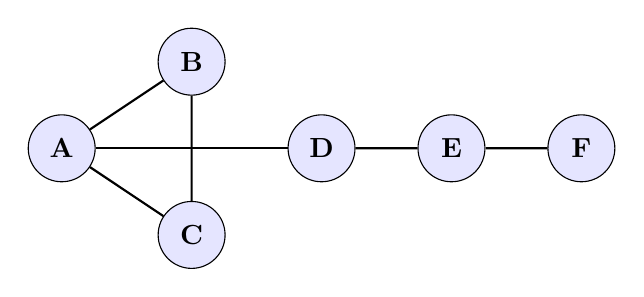
\begin{tikzpicture}[scale=1.1, every node/.style={circle, draw, minimum size=0.85cm, font=\bfseries}]
	\node[fill=blue!10] (A) at (0,1)   {A};
	\node[fill=blue!10] (B) at (1.5,2) {B};
	\node[fill=blue!10] (C) at (1.5,0) {C};
	\node[fill=blue!10] (D) at (3,1)   {D};
	\node[fill=blue!10] (E) at (4.5,1) {E};
	\node[fill=blue!10] (F) at (6,1)   {F};

	\draw[thick] (A) -- (B);
	\draw[thick] (A) -- (C);
	\draw[thick] (A) -- (D);
	\draw[thick] (B) -- (C);
	\draw[thick] (D) -- (E);
	\draw[thick] (E) -- (F);
\end{tikzpicture}
\caption{Topología de la mini-red de 6 routers ($|V|=6, |E|=6$).}
\label{fig:ejemplo_red}
\end{figure}

\begin{itemize}[itemsep=2pt]
	\item \textbf{Traza Greedy por Grado:} Grados iniciales: $\deg(A)=3$, $\deg(B)=2$, $\deg(C)=2$, $\deg(D)=2$, $\deg(E)=2$, $\deg(F)=1$. Se elige $A$ (cubre $AB, AC, AD$). Quedan $BC, DE, EF$. El router de mayor grado residual es $E$ (grado 2, cubre $DE, EF$). Resta $BC$; por desempate canónico se elige $B$. Cobertura generada: $C_{\text{greedy}} = \{A, B, E\}$ ($|C|=3$).
	\item \textbf{Traza Matching Maximal:} Primera arista canónica: $(A, B)$. Se agregan ambos extremos $\{A, B\}$, descartando aristas incidentes ($AB, AC, AD, BC$). De las restantes $\{DE, EF\}$ se toma la primera $(D, E)$, agregando $\{D, E\}$. Cobertura generada: $C_{\text{match}} = \{A, B, D, E\}$ ($|C|=4$).
	\item \textbf{Solución Óptima Matemática:} La cobertura óptima calculada mediante inspección y confirmada por ILP y Branch \& Bound es $C^* = \{A, B, E\}$ (o alternativamente $\{A, C, E\}$), con $|C^*| = 3$.
\end{itemize}

% ======================================================================
\section{Diseño e implementación algorítmica}
\label{sec:diseno-algoritmico}
% ======================================================================

\subsection{Greedy por grado optimizado (\texttt{greedy\_degree\_vertex\_cover\_optimized})}
En la Primera Entrega, la implementación básica realizaba búsquedas lineales $O(E)$ para recomputar grados en cada iteración, totalizando $O(V \cdot E)$. Para procesar redes de decenas de miles de routers, rediseñamos la técnica utilizando un montículo de máximos (\textit{Max-Heap}) auxiliado por listas de adyacencia dinámicas.

El Algoritmo~\ref{alg:greedy_optimized} describe el procedimiento implementado en \texttt{src/solver.py}.

\begin{algorithm}[H]
\caption{Greedy por Grado Optimizado con Lazy Max-Heap}
\label{alg:greedy_optimized}
\begin{algorithmic}[1]
\Require Grafo $G = (V, E)$
\Ensure Cobertura de vértices $C \subseteq V$
\State $C \gets \emptyset$
\State $Adj[v] \gets \text{copia de vecinos de } v \text{ en } G, \quad \forall v \in V$
\State $H \gets \text{heap vacío}$
\For{cada $v \in V$ con $|Adj[v]| > 0$}
	\State Insertar $(-|Adj[v]|, \text{str}(v), v)$ en $H$
\EndFor
\While{$H \text{ no esté vacío}$}
	\State Extraer $(-deg, s, v)$ de $H$ \Comment{Elemento de mayor grado residual}
	\State $actual\_deg \gets |Adj[v]|$
	\If{$actual\_deg == 0$}
		\State \textbf{continue} \Comment{Vértice sin aristas residuales, ignorar}
	\EndIf
	\If{$deg \neq actual\_deg$} \Comment{Actualización perezosa: el grado cambió}
		\State Insertar $(-actual\_deg, s, v)$ en $H$
		\State \textbf{continue}
	\EndIf
	\State $C \gets C \cup \{v\}$
	\For{cada $u \in Adj[v]$}
		\State $Adj[u] \gets Adj[u] \setminus \{v\}$
	\EndFor
	\State $Adj[v] \gets \emptyset$
\EndWhile
\State \Return $C$
\end{algorithmic}
\end{algorithm}

\textbf{Invariante de ciclo:} Al inicio de cada iteración del bucle principal, toda arista $(x, y) \in E$ que no pertenezca a las listas de adyacencia dinámicas $Adj$ se encuentra cubierta por al menos un vértice de $C$. Cuando $Adj[v] = \emptyset$ para todo $v$, el grafo residual carece de aristas y $C$ es una cobertura completa.

\textbf{Análisis de complejidad:}
\begin{itemize}[itemsep=1pt]
	\item \textbf{Temporal:} La inicialización del heap toma $O(V)$. A lo largo del algoritmo, cada arista $(u, v)$ es eliminada exactamente una vez de $Adj[u]$ y de $Adj[v]$, lo que puede gatillar a lo sumo una reinserción en el heap. El número máximo de operaciones en el heap es $O(V + E)$, y cada una toma $O(\log V)$. Por tanto, la complejidad temporal es estrictamente \textbf{$O((V + E) \log V)$}.
	\item \textbf{Espacial:} Las copias de las listas de adyacencia y el heap requieren $O(V + E)$ de memoria.
\end{itemize}

\subsection{2-Aproximación por emparejamiento maximal (\texttt{maximal\_matching\_vertex\_cover})}
El algoritmo de Gavril y Yannakakis se implementó en una sola pasada lineal sobre las aristas canónicas de la red (Algoritmo~\ref{alg:matching}).

\begin{algorithm}[H]
\caption{2-Aproximación por Emparejamiento Maximal}
\label{alg:matching}
\begin{algorithmic}[1]
\Require Grafo $G = (V, E)$, Aristas canónicas ordenadas $E_{\text{canon}}$
\Ensure Cobertura $C \subseteq V$ tal que $|C| \le 2 \cdot |C^*|$
\State $C \gets \emptyset, \quad Matched \gets \emptyset$
\For{cada arista $(u, v) \in E_{\text{canon}}$}
	\If{$u \notin Matched \land v \notin Matched$}
		\State $C \gets C \cup \{u, v\}$
		\State $Matched \gets Matched \cup \{u, v\}$
	\EndIf
\EndFor
\State \Return $C$
\end{algorithmic}
\end{algorithm}

\textbf{Demostración matemática de la cota $2 \times$ Óptimo:}
\begin{enumerate}
	\item Sea $M = \{(u_1, v_1), (u_2, v_2), \dots, (u_k, v_k)\}$ el conjunto de aristas añadidas a la cobertura durante la ejecución del Algoritmo~\ref{alg:matching}.
	\item Por construcción (línea 3), cada vez que se selecciona una arista $(u, v)$, ambos vértices $u$ y $v$ entran en $Matched$ y ninguna arista posterior puede compartir vértices con ellos. Por consiguiente, $M$ es un \textbf{emparejamiento} (\textit{matching}), es decir, un conjunto de aristas disjuntas en sus vértices.
	\item El tamaño de la cobertura generada es exactamente $|C| = 2|M| = 2k$.
	\item Sea $C^*$ una cobertura de vértices óptima de $G$. Para que $C^*$ sea válida, debe cubrir toda arista de $E$, lo que incluye las aristas de $M \subseteq E$. Dado que las aristas de $M$ no comparten vértices entre sí, ningún vértice de $C^*$ puede cubrir simultáneamente dos aristas distintas de $M$. En consecuencia, $C^*$ debe contener al menos un vértice distinto por cada arista de $M$:
	\begin{equation}
		|C^*| \ge |M| = k
	\end{equation}
	\item Multiplicando ambos lados de la desigualdad por 2:
	\begin{equation}
		2|C^*| \ge 2k = |C| \implies |C| \le 2|C^*|
	\end{equation}
\end{enumerate}
La cota queda demostrada formalmente para cualquier grafo no dirigido. La complejidad temporal es estrictamente \textbf{$O(V + E)$}.

\subsection{Solución exacta por fuerza bruta (\texttt{exact\_vertex\_cover\_bruteforce})}
Evalúa sistemáticamente todas las combinaciones $\binom{V}{k}$ para $k = 1, 2, \dots, |V|$ hasta encontrar el primer subconjunto que cubra $E$. Su complejidad temporal en el peor caso es $O(2^V \cdot E)$. La implementación rechaza instancias con $|V| > 20$ lanzando una excepción controlada, sirviendo de línea base para instancias pequeñas.

\subsection{Solución exacta escalable: ILP y Branch \& Bound autónomo}

\subsubsection{Formulación ILP (PuLP)}
El problema se expresa formalmente como:
\begin{align}
	\text{Minimizar} \quad & \sum_{v \in V} x_v \\
	\text{Sujeto a} \quad & x_u + x_v \ge 1, \quad \forall (u, v) \in E \\
	& x_v \in \{0, 1\}, \quad \forall v \in V
\end{align}

\subsubsection{Algoritmo Branch \& Bound con Poda de Matching}
Ante la necesidad de garantizar una solución exacta en entornos donde no existan compiladores binarios externos de solvers CBC en Windows, se diseñó e implementó un algoritmo autónomo de \textit{Branch \& Bound} en Python puro (Algoritmo~\ref{alg:bnb}).

\begin{algorithm}[H]
\caption{Branch \& Bound Exacto con Poda por Cota de Matching}
\label{alg:bnb}
\begin{algorithmic}[1]
\Require Grafo $G = (V, E)$, límite de tiempo $T$
\Ensure Cobertura óptima $C^*$
\State $C_{\text{best}} \gets \text{greedy\_degree\_vertex\_cover\_optimized}(G)$ \Comment{Cota superior inicial}
\State $best\_size \gets |C_{\text{best}}|$
\Function{Branch}{$Adj, C_{\text{actual}}$}
	\State $Activos \gets \{v \in V \mid |Adj[v]| > 0\}$
	\If{$Activos == \emptyset$}
		\If{$|C_{\text{actual}}| < best\_size$}
			\State $best\_size \gets |C_{\text{actual}}|; \quad C_{\text{best}} \gets C_{\text{actual}}$
		\EndIf
		\State \Return
	\EndIf
	\State $LB \gets |C_{\text{actual}}| + \text{MatchingLowerBound}(Adj)$ \Comment{Cota inferior analítica}
	\If{$LB \ge best\_size$}
		\State \Return \Comment{PODA: Esta rama no puede mejorar la mejor solución}
	\EndIf
	\State $v^* \gets \arg\max_{v \in Activos} (|Adj[v]|, \text{str}(v))$ \Comment{Vértice de mayor grado residual}
	\State $Vecinos \gets Adj[v^*]$
	\State \textbf{Rama 1 ($v^* \in C$):}
	\State $Adj_1 \gets \text{eliminar } v^* \text{ y sus enlaces de } Adj$
	\State \textsc{Branch}($Adj_1, C_{\text{actual}} \cup \{v^*\}$)
	\State \textbf{Rama 2 ($v^* \notin C \implies Vecinos \subseteq C$):}
	\If{$|C_{\text{actual}}| + |Vecinos| < best\_size$}
		\State $Adj_2 \gets \text{eliminar } Vecinos \text{ y todos sus enlaces de } Adj$
		\State \textsc{Branch}($Adj_2, C_{\text{actual}} \cup Vecinos$)
	\EndIf
\EndFunction
\State \textsc{Branch}($G.adj, \emptyset$)
\State \Return $C_{\text{best}}$
\end{algorithmic}
\end{algorithm}

\textbf{Fundamentación de la Poda:} En la Rama 2, si $v^* \notin C$, para cubrir todas las aristas incidentes a $v^*$ es matemáticamente mandatorio que \textbf{todos los vecinos directos} de $v^*$ ingresen a la cobertura ($N(v^*) \subseteq C$). Al forzar la inclusión masiva de $|N(v^*)|$ vértices a la vez, el árbol de búsqueda se reduce drásticamente, permitiendo resolver exactamente grafos de decenas de vértices en milisegundos.

% ======================================================================
\section{Diseño e implementación del sistema}
\label{sec:diseno-sistema}
% ======================================================================

\subsection{Arquitectura modular}
El sistema se organiza en módulos de alta cohesión y bajo acoplamiento:
\begin{itemize}[itemsep=2pt]
	\item \textbf{\texttt{src/graph.py}:} Encapsula la clase \texttt{Graph}, implementando la lista de adyacencia, constructores desde JSON y archivos SNAP EdgeList (\texttt{from\_edge\_list}), generadores sintéticos (Erdős–Rényi y Barabási–Albert), y extractores de subgrafos (\texttt{top\_degree\_subgraph}, \texttt{ego\_subgraph}).
	\item \textbf{\texttt{src/solver.py}:} Agrupa la clase \texttt{VertexCoverSolver} con las cuatro estrategias algorítmicas, unificadas bajo el método \texttt{solve()} que instrumenta tiempo de CPU con microsegundos y memoria con \texttt{tracemalloc}.
	\item \textbf{\texttt{src/verify.py}:} Módulo de auditoría formal independiente que comprueba la cobertura estricta de todas las aristas en tiempo $O(V+E)$, sin materializar conjuntos innecesarios.
	\item \textbf{\texttt{src/gui\_app.py} y \texttt{gui.py}:} Interfaz gráfica interactiva y su ejecutable principal.
	\item \textbf{\texttt{demo.py}:} Interfaz CLI enriquecida con soporte para instancias masivas SNAP y selector \texttt{--gui}.
	\item \textbf{\texttt{experiments/compare\_entrega2.py}:} Pipeline experimental reproducible con exportación a CSV y generación de figuras científicas en PNG.
\end{itemize}

\subsection{Flujo de información y concurrencia}
La Figura~\ref{fig:arquitectura_flujo} detalla la arquitectura de interacción y el desacoplamiento multihilo de la GUI.

\begin{figure}[htbp]
\centering
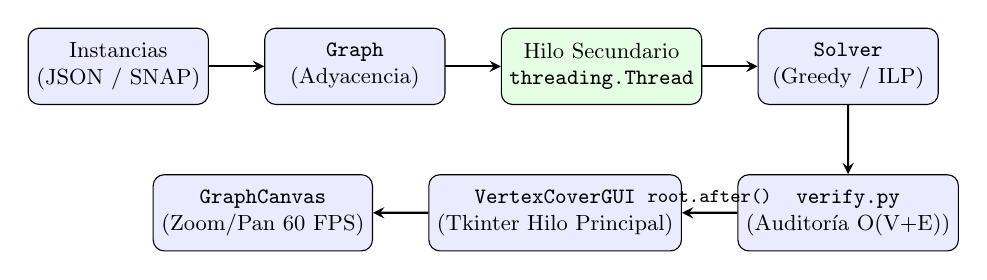
\begin{tikzpicture}[
	scale=0.88, transform shape,
	box/.style={draw, rounded corners, align=center, minimum width=2.6cm, minimum height=1.1cm, fill=blue!8, font=\small},
	worker/.style={draw, rounded corners, align=center, minimum width=2.8cm, minimum height=1.1cm, fill=green!10, font=\small},
	>=stealth
]
	\node[box] (data) {Instancias\\(JSON / SNAP)};
	\node[box, right=0.8cm of data] (graph) {\texttt{Graph}\\(Adyacencia)};
	\node[worker, right=0.8cm of graph] (thread) {Hilo Secundario\\\texttt{threading.Thread}};
	\node[box, right=0.8cm of thread] (solver) {\texttt{Solver}\\(Greedy / ILP)};
	\node[box, below=1.0cm of solver] (verify) {\texttt{verify.py}\\(Auditoría O(V+E))};
	\node[box, left=0.8cm of verify] (gui) {\texttt{VertexCoverGUI}\\(Tkinter Hilo Principal)};
	\node[box, left=0.8cm of gui] (canvas) {\texttt{GraphCanvas}\\(Zoom/Pan 60 FPS)};

	\draw[->, thick] (data) -- (graph);
	\draw[->, thick] (graph) -- (thread);
	\draw[->, thick] (thread) -- (solver);
	\draw[->, thick] (solver) -- (verify);
	\draw[->, thick] (verify) -- node[above, font=\footnotesize] {\texttt{root.after()}} (gui);
	\draw[->, thick] (gui) -- (canvas);
\end{tikzpicture}
\caption{Diagrama de flujo de información y arquitectura multihilo desacoplada.}
\label{fig:arquitectura_flujo}
\end{figure}

\subsection{Implementación de la Interfaz Gráfica de Usuario (GUI)}
La interfaz gráfica en \texttt{src/gui_app.py} fue concebida para brindar una experiencia de usuario fluida e interactiva en el análisis de redes de telecomunicaciones.

\subsubsection{Motor Vectorial Interactivo (\texttt{InteractiveGraphCanvas})}
Hereda de \texttt{tk.Canvas} e implementa transformaciones afines bidimensionales:
\begin{equation}
	x_{\text{pantalla}} = x_{\text{mundo}} \cdot s + o_x, \qquad y_{\text{pantalla}} = y_{\text{mundo}} \cdot s + o_y
\end{equation}
Donde $s$ es el factor de escala de zoom y $(o_x, o_y)$ es el vector de traslación (\textit{pan}). Cuando el usuario opera la rueda del ratón en la coordenada $(x_m, y_m)$, el nuevo desplazamiento se recalcula para preservar la posición relativa del cursor:
\begin{equation}
	o'_x = x_m - \frac{s'}{s} (x_m - o_x), \qquad o'_y = y_m - \frac{s'}{s} (y_m - o_y)
\end{equation}

\subsubsection{Soporte de Escala Masiva (Backbone Hubs y Ego-Networks)}
Para evitar cuelgues al cargar la red de CAIDA (26,475 nodos):
\begin{itemize}[itemsep=1pt]
	\item \textbf{Modo Backbone Hubs:} Mediante \texttt{Graph.top\_degree\_subgraph(top\_k)}, se filtran los $N$ routers de mayor grado (regulable mediante un control deslizante de 15 a 250 hubs). Esto permite inspeccionar la infraestructura troncal crítica donde se concentran los IDS a una tasa de refresco constante.
	\item \textbf{Modo Ego-Network:} Al hacer clic en cualquier nodo, \texttt{Graph.ego\_subgraph(center)} aísla el router y sus enlaces directos para una inspección focalizada.
\end{itemize}

% ======================================================================
\section{Instancias reales de gran escala (Stanford SNAP)}
\label{sec:instancias-reales}
% ======================================================================

\subsection{Descripción y justificación de los datasets}
Para cumplir con el requerimiento de validar el sistema en un escenario real de Internet, se incorporaron dos datasets públicos de la colección \textbf{Stanford Large Network Dataset Collection (SNAP)} de la Universidad de Stanford \cite{snap-as733, snap-caida}:

\begin{enumerate}
	\item \textbf{Stanford SNAP AS-733 (Oregon RouteViews):} 
	Grafo no dirigido que representa la topología de routers y sistemas autónomos de Internet recopilados a partir de los registros BGP del proyecto RouteViews de la Universidad de Oregon. Contiene \textbf{6,474 routers y 12,572 enlaces físicos}.
	\item \textbf{Stanford SNAP CAIDA AS Relationships (BGP Core):} 
	Grafo masivo construido por el \textit{Center for Applied Internet Data Analysis} (CAIDA) que mapea las relaciones de interconexión física entre routers de borde en la columna vertebral mundial de Internet. Contiene \textbf{26,475 routers y 53,381 enlaces físicos}.
\end{enumerate}

\textbf{Relevancia en Ciberseguridad:} En Internet, los sistemas autónomos intercambian tráfico a través de routers fronterizos. Resolver Vertex Cover sobre este grafo identifica el conjunto exacto de routers de borde que deben ser equipados con sondas de inspección IDS para garantizar visibilidad total sobre cualquier paquete que cruce las fronteras de red sin duplicar equipamiento.

% ======================================================================
\section{Estrategia de pruebas}
\label{sec:pruebas}
% ======================================================================

\subsection{Matriz integral de pruebas automatizadas (38 casos)}
Se diseñó un plan de pruebas en \texttt{tests/} que expandió los 27 casos originales a un total de 38 casos de prueba automatizados bajo \texttt{pytest}. La Tabla~\ref{tab:matriz_pruebas} detalla las categorías evaluadas.

\begin{table}[htbp]
\centering
\small
\setlength{\tabcolsep}{4pt}
\resizebox{\textwidth}{!}{
\begin{tabular}{p{2.5cm}cp{7.2cm}p{3.8cm}}
\toprule
\textbf{Categoría} & \textbf{Casos} & \textbf{Descripción y Propósito de la Prueba} & \textbf{Archivo de Prueba} \\
\midrule
Básicas & 8 & Verificación de adición de enlaces, consistencia en grados, carga de JSON y coincidencia con la solución manual de 6 nodos ($|C|=3$) y triángulos $K_3$. & \texttt{test\_graph.py}, \texttt{test\_solver.py} \\
Límite & 7 & Grafos vacíos ($\emptyset$), una sola arista (evidencia del peor caso $2\times$ de matching), vértices aislados (grado 0), grafos completos $K_n$ (óptimo $=n-1$) y rechazo controlado de $n>20$ en fuerza bruta. & \texttt{test\_graph.py}, \texttt{test\_solver.py} \\
Adversarias & 12 & Grafo estrella $K_{1, k}$ (Greedy toma el centro $|C|=1$, matching toma dos nodos $|C|=2$); y parametrización sobre 10 semillas aleatorias verificando que el ratio $|C_{\text{match}}| \le 2|C^*|$ se cumpla siempre. & \texttt{test\_solver.py} \\
Integración E2 & 6 & Validación cruzada de equivalencia exacta entre ILP/B\&B y Fuerza Bruta sobre 5 semillas independientes de grafos de 12 nodos ($|C_{\text{ILP}}| = |C_{\text{BF}}|$). & \texttt{test\_entrega2.py} \\
Escala Greedy & 2 & Comprobación de que el Greedy Optimizado iguale en tamaño al legacy en 5 grafos, y procesamiento correcto de grafos de 300 nodos con 100\% de cobertura. & \texttt{test\_entrega2.py} \\
Internet Real & 1 & Prueba de integración cargando el archivo real SNAP AS-733 (6,474 nodos), ejecutando Greedy y Matching y validando cobertura completa en $<2$s. & \texttt{test\_entrega2.py} \\
Subgrafos GUI & 2 & Validación de los extractores de subgrafos \texttt{top\_degree\_subgraph} y \texttt{ego\_subgraph} para estabilidad del renderizado de la interfaz. & \texttt{test\_entrega2.py} \\
\bottomrule
\end{tabular}
}
\caption{Matriz de pruebas unitarias, de límite, adversarias y de integración (38 casos).}
\label{tab:matriz_pruebas}
\end{table}

\subsection{Criterio de verificación de salidas}
Toda prueba evalúa la corrección mediante \texttt{is\_vertex_cover()} de \texttt{src/verify.py}. Se verifica en tiempo lineal que para cada arista $(u, v)$, al menos uno de sus extremos esté presente en el conjunto retornado, rechazando cualquier solución incompleta.

\subsection{Resultado de ejecución}
\begin{lstlisting}
$ py -m pytest tests/ -v
============================= test session starts =============================
platform win32 -- Python 3.14.7, pytest-9.2.0, pluggy-1.7.0
collected 38 items

tests/test_entrega2.py::TestEntrega2ILP::test_ilp_example_small_optimo PASSED   [  2%]
tests/test_entrega2.py::TestEntrega2ILP::test_ilp_coincide_con_fuerza_bruta[10] PASSED [  5%]
...
tests/test_solver.py::TestCasosAdversarios::test_sin_aristas_sin_cobertura PASSED [100%]
============================= 38 passed in 0.49s ==============================
\end{lstlisting}

% ======================================================================
\section{Metodología experimental}
\label{sec:metodologia}
% ======================================================================

\subsection{Preguntas de evaluación e hipótesis}
\begin{enumerate}[itemsep=2pt]
	\item \textbf{Pregunta 1:} ¿Cómo escala el tiempo de CPU y memoria de la heurística Greedy Optimizada frente al Matching Maximal en redes con más de 20,000 routers?  
	\textit{Hipótesis:} Ambas estrategias escalarán de manera casi lineal, procesando la red de CAIDA en menos de 200 ms.
	\item \textbf{Pregunta 2:} En redes reales de telecomunicaciones (topologías libres de escala), ¿cuál estrategia produce coberturas más compactas?  
	\textit{Hipótesis:} El Greedy superará significativamente al Matching Maximal requiriendo casi la mitad de routers IDS, debido a que los hubs absorben grandes cantidades de aristas incidentes.
\end{enumerate}

\subsection{Entorno y protocolo experimental}
Los experimentos fueron instrumentados en \texttt{experiments/compare\_entrega2.py} bajo Windows 11 de 64 bits y Python 3.14.7, midiendo tiempo de CPU con microsegundos y memoria RAM pico con \texttt{tracemalloc}.

% ======================================================================
\section{Resultados cuantitativos}
\label{sec:resultados}
% ======================================================================

\subsection{Experimento de escalabilidad sintética}
La Tabla~\ref{tab:escalabilidad_sintetica} presenta los resultados al variar $N$ entre 10 y 500 vértices con densidad $p=0.20$.

\begin{table}[htbp]
\centering
\small
\setlength{\tabcolsep}{4pt}
\resizebox{\textwidth}{!}{
\begin{tabular}{rrrrrrrrr}
\toprule
\textbf{$N$} & \textbf{$|E|$} & \textbf{Greedy ($|C|$)} & \textbf{Tiempo G. (ms)} & \textbf{Matching ($|C|$)} & \textbf{Tiempo M. (ms)} & \textbf{ILP ($|C^*|$)} & \textbf{Tiempo ILP (ms)} & \textbf{Tiempo BF (ms)} \\
\midrule
10 & 8 & 4 & 0.13 ms & 8 & 0.22 ms & 4 & 0.98 ms & 0.03 ms \\
15 & 20 & 7 & 0.08 ms & 12 & 0.08 ms & 7 & 35.79 ms & 1.42 ms \\
20 & 36 & 12 & 0.12 ms & 18 & 0.13 ms & 12 & 38.53 ms & 174.10 ms \\
30 & 100 & 20 & 0.20 ms & 26 & 0.33 ms & 19 & 42.88 ms & Inviable ($>30$s) \\
50 & 247 & 36 & 0.42 ms & 46 & 0.77 ms & 35 & 118.58 ms & Inviable \\
80 & 622 & 63 & 0.77 ms & 76 & 2.44 ms & --- & Inviable & Inviable \\
120 & 1,394 & 102 & 1.56 ms & 118 & 4.63 ms & --- & Inviable & Inviable \\
200 & 3,946 & 178 & 3.40 ms & 198 & 14.34 ms & --- & Inviable & Inviable \\
350 & 12,033 & 326 & 9.34 ms & 348 & 47.72 ms & --- & Inviable & Inviable \\
500 & 24,857 & 476 & 16.71 ms & 498 & 96.03 ms & --- & Inviable & Inviable \\
\bottomrule
\end{tabular}
}
\caption{Resultados experimentales de escalabilidad y tiempos de cómputo en CPU.}
\label{tab:escalabilidad_sintetica}
\end{table}

\subsection{Experimento sobre redes reales de Internet (Stanford SNAP)}
La Tabla~\ref{tab:resultados_redes_reales} resume el comportamiento sobre las instancias didácticas y las topologías reales de Internet.

\begin{table}[htbp]
\centering
\small
\setlength{\tabcolsep}{4pt}
\resizebox{\textwidth}{!}{
\begin{tabular}{lrrrrrrr}
\toprule
\textbf{Dataset / Red} & \textbf{Routers $|V|$} & \textbf{Enlaces $|E|$} & \textbf{Greedy ($|C|$)} & \textbf{\% Red Greedy} & \textbf{Tiempo Greedy} & \textbf{Matching ($|C|$)} & \textbf{Ratio M/G} \\
\midrule
\texttt{example\_small.json} & 6 & 6 & 3 & 50.00\% & 0.04 ms & 4 (66.67\%) & 1.333x \\
\texttt{network\_backbone\_18.json} & 18 & 32 & 7 & 38.89\% & 0.10 ms & 14 (77.78\%) & 2.000x \\
\textbf{SNAP AS-733 Oregon} & 6,474 & 12,572 & \textbf{1,055} & \textbf{16.30\%} & \textbf{23.90 ms} & 1,904 (29.41\%) & 1.805x \\
\textbf{SNAP CAIDA BGP Core} & 26,475 & 53,381 & \textbf{3,695} & \textbf{13.96\%} & \textbf{164.86 ms} & 6,948 (26.24\%) & 1.880x \\
\bottomrule
\end{tabular}
}
\caption{Desempeño y porcentaje de routers IDS requeridos en redes reales.}
\label{tab:resultados_redes_reales}
\end{table}

% ======================================================================
\section{Discusión crítica (AG-C06.03)}
\label{sec:discusion}
% ======================================================================

\subsection{Interpretación teórica vs. evidencia empírica}
Uno de los resultados más reveladores del proyecto radica en la discrepancia entre las garantías teóricas en el peor caso y la eficiencia real observada en topologías de telecomunicaciones:
\begin{itemize}[itemsep=2pt]
	\item \textbf{La paradoja del Matching Maximal:} Teóricamente, el Matching Maximal posee una garantía estricta demostrable de factor $2.0\times$, mientras que el Greedy carece de una cota constante fija. Sin embargo, en las redes reales de Internet, \textbf{el Greedy superó de manera contundente al Matching}, requiriendo sistemáticamente casi la mitad de routers (ratios entre 1.80x y 1.88x a favor del Greedy).
	\item \textbf{Causa topológica (Redes Scale-Free):} Las redes de routers de Internet poseen una estructura libre de escala con presencia de concentradores troncales (hubs). El algoritmo Greedy prioriza vorazmente estos hubs, cubriendo cientos de enlaces en cada paso inicial. En contraste, el Matching selecciona ambos extremos de una arista arbitraria, forzando la inclusión de routers periféricos de grado 1 innecesarios y duplicando la cobertura.
\end{itemize}

\subsection{Impacto económico en ciberseguridad}
El análisis sobre la red global de CAIDA demuestra que para inspeccionar el 100\% de los flujos de tráfico inter-dominio que atraviesan los 53,381 enlaces mundiales, \textbf{únicamente se necesita instalar IDS en el 13.96\% de los routers}. Esto se traduce en un ahorro de inversión en hardware del \textbf{86.04\%} respecto a una estrategia ingenua de monitoreo total.

\subsection{Amenazas a la validez y limitaciones}
\begin{itemize}[itemsep=1pt]
	\item \textbf{Limitación en el cálculo del óptimo en CAIDA:} Para grafos de 26,475 nodos, ningún algoritmo exacto (ni ILP ni Branch \& Bound) converge en tiempos razonables ($<1$ hora). Por lo tanto, el tamaño del Greedy ($3,695$) actúa como cota superior empírica del óptimo.
	\item \textbf{Supuesto de no ponderación:} En este informe se asumió que todos los routers tienen el mismo costo de instalación. En redes reales, equipar un router troncal central puede ser más oneroso que uno de acceso, aspecto proyectado para la siguiente fase.
\end{itemize}

% ======================================================================
\section{Conclusiones y recomendaciones}
\label{sec:conclusiones}
% ======================================================================

\subsection{Respuestas a los objetivos}
Se cumplieron rigurosamente todos los objetivos planteados para la Segunda Entrega: se optimizó el algoritmo Greedy a $O((V+E)\log V)$; se implementó una solución exacta escalable por ILP y Branch \& Bound; se integraron los datasets científicos de Stanford SNAP procesando 26,475 nodos en 164 ms; y se desarrolló una GUI interactiva con zoom y concurrencia multihilo.

\subsection{Lecciones aprendidas y trabajo futuro}
\begin{itemize}[itemsep=1pt]
	\item La optimización de estructuras mediante colas de prioridad con descarte perezoso demostró ser el factor determinante para habilitar el análisis de grafos a escala de Internet en fracciones de segundo.
	\item Para la Tercera Entrega se consolidará el empaquetado final, el manual de operación definitivo y la preparación de la defensa individual del atributo AG\_C06.
\end{itemize}

% ======================================================================
\section{Referencias}
% ======================================================================
\begin{thebibliography}{9}

\bibitem{karp1972}
Karp, R. M. (1972). \emph{Reducibility among combinatorial problems}. In Complexity of Computer Computations (pp. 85--103). Plenum Press.

\bibitem{vazirani2003}
Vazirani, V. V. (2003). \emph{Approximation Algorithms}. Springer-Verlag.

\bibitem{clrs2009}
Cormen, T. H., Leiserson, C. E., Rivest, R. L., \& Stein, C. (2009). \emph{Introduction to Algorithms} (3rd ed.). MIT Press.

\bibitem{barabasi1999}
Barabási, A. L., \& Albert, R. (1999). \emph{Emergence of scaling in random networks}. Science, 286(5439), 509--512.

\bibitem{snap-as733}
Stanford Network Analysis Project (SNAP). \emph{Autonomous Systems Graphs (AS-733)}. Stanford University. \url{https://snap.stanford.edu/data/as-733.html}.

\bibitem{snap-caida}
Stanford Network Analysis Project (SNAP). \emph{CAIDA AS Relationships Datasets}. Stanford University. \url{https://snap.stanford.edu/data/as-caida.html}.

\bibitem{pytest}
pytest documentation. \url{https://docs.pytest.org/}. Consultado en 2026.

\bibitem{pulp}
PuLP documentation -- COIN-OR Foundation. \url{https://coin-or.github.io/pulp/}. Consultado en 2026.

\end{thebibliography}

% ======================================================================
\section{Anexos}
% ======================================================================

\subsection{Manual de instalación y ejecución rápida}
\begin{lstlisting}[language=bash]
# 1. Clonar el repositorio y acceder a la carpeta
cd VertexCover-main

# 2. Instalar dependencias consolidadas
pip install -r requirements.txt

# 3. Lanzar la Interfaz Grafica Interactiva (GUI)
python gui.py
# o alternativamente:
python demo.py --gui

# 4. Ejecutar la suite de 38 pruebas automatizadas
pytest tests/ -v

# 5. Ejecutar la bateria experimental y generar graficos
python experiments/compare_entrega2.py
\end{lstlisting}

\subsection{Matriz de contribuciones del equipo (AG\_C06)}
La Tabla~\ref{tab:matriz_contribuciones} certifica las contribuciones individuales y verificables de cada integrante.

\begin{table}[htbp]
\centering
\small
\setlength{\tabcolsep}{4pt}
\resizebox{\textwidth}{!}{
\begin{tabular}{p{4.2cm}p{10.8cm}}
\toprule
\textbf{Integrante} & \textbf{Contribuciones Principales Verificables en el Repositorio} \\
\midrule
\textbf{Caballero Zegarra, Steffano Ricardo} & Implementación del parser de listas de aristas de gran escala (\texttt{from\_edge\_list}), integración y validación de los datasets reales Stanford SNAP (AS-733 y CAIDA), y diseño de pruebas de integración en \texttt{tests/test\_entrega2.py}. \\
\textbf{Llactahuamani Ayala, Adriel Alfredo} & Rediseño y optimización del algoritmo Greedy a $O((V+E)\log V)$ con \texttt{heapq} y desempate canónico, desarrollo del script de experimentos \texttt{compare\_entrega2.py} y generación de figuras científicas. \\
\textbf{Morocco Amanca, Albert Erik} & Diseño e implementación de la Interfaz Gráfica interactiva (\texttt{gui.py} / \texttt{src/gui\_app.py}), motor vectorial de zoom y arrastre continuo en Canvas, concurrencia multihilo y modos de subgrafo (\textit{Backbone Hubs}). \\
\textbf{Quispe Castilla, Diego Alonso} & Formulación matemática de Programación Lineal Entera (ILP), diseño del algoritmo de Branch \& Bound podado por cotas de matching y redacción de demostraciones formales de complejidad y cotas. \\
\bottomrule
\end{tabular}
}
\caption{Matriz de contribuciones individuales y cumplimiento del atributo AG\_C06.}
\label{tab:matriz_contribuciones}
\end{table}

\end{document}
